% -*- TeX-master: "main"; fill-column: 72 -*-

\section{Introduction}
\label{intro}

In the context of SBML, ``hierarchical model composition'' refers to the
ability to include models as submodels inside other models. The goal is
to support the ability of modelers and software tools to do such things
as (1) decompose larger models into smaller ones, as a way to manage
model complexity; (2) incorporate multiple instances of the same
component model within one or more enclosing models, to avoid literal
duplication of repeated elements; and (3) create libraries of reusable,
tested models, much as is done in software development and other
engineering fields.

SBML Level 3 Core has no direct support for allowing a model to include
other models as submodels.  Software tools either have to implement
their own schemes outside of SBML, or (in principle) could use
annotations to augment a plain SBML Level~3 model with the necessary
information to allow a software tool to compose a model out of
submodels.  However, such solutions would be proprietary and
tool-specific, and not conducive to interoperability.  There is a clear
need for an official SBML language facility for hierarchical model
composition.

This document describes a specification for an SBML Level~3 package that
provides exactly such a facility.  \fig{fig1} illustrates some of the
scenarios targeted by this package.

\begin{figure}[hb]
  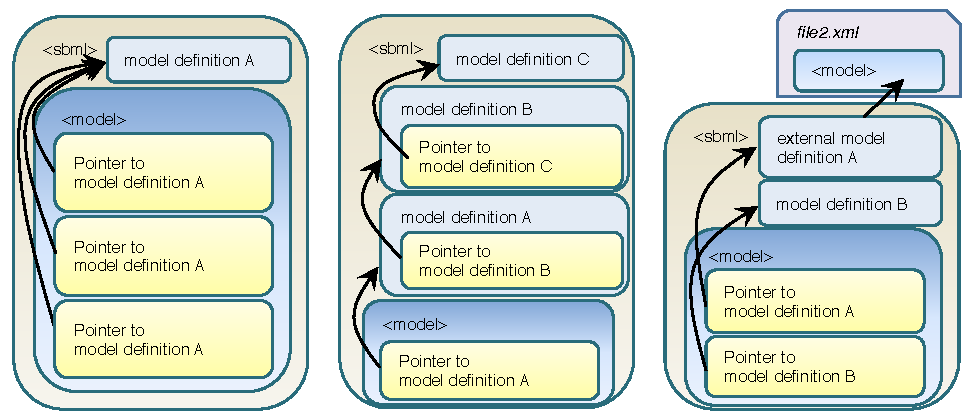
\includegraphics{figs/figure1}
  \caption{Three different examples of model composition scenarios.
    From left to right: (1) a model composed of multiple instances of a
    single, internally-defined submodel definition; (2) a model composed
    of a submodel that is itself composed of submodels; and (3) a model
    composed of submodels, one of which is defined in an external file.}
  \label{fig1}
\end{figure}

The effort to create a hierarchical model composition mechanism in SBML
has a long history, which we summarize in the next section.  It has also
been known by different names.  Originally, it was called
\emph{modularity} because it allows a model to be divided into
structural and conceptual modules.  It was renamed \emph{model
  composition} when it became apparent that the name ``modularity'' was
too-easily confused with other notions modularity, particularly
XHTML~1.1~\cite{} modularity (which concerns decomposition into separate
files).  To make clear that the purpose is structural \emph{model}
composition, regardless of whether the components are stored in separate
files, the SBML community adopted the name SBML \emph{Hierarchical Model
  Composition}.

To support a variety of composition scenarios, this package provides for
optional black-box encapsulation by means of defined data communication
interfaces (here called \emph{ports}).  In addition, it also separates
model \emph{definitions} (i.e., blueprints, or templates) from
\emph{instances} of those definitions, it supports optional external
file storage, and it allows recursive model decomposition with arbitrary
submodel nesting.


\subsection{Proposal corresponding to this package specification}

This Hierarchical Model Composition package specification for SBML
Level~3 Version~1 Core is based on the proposal by the same authors,
located at the following URL:

\begin{quote}\small
  \url{https://sbml.svn.sf.net/svnroot/sbml/trunk/specifications/sbml-level-3/version-1/comp}
\end{quote}

The tracking number in the SBML issue tracking system~\cite{t} for
Hierarchical Model Composition package activities is 2404771.  The
version of the proposal used as the starting point for this
specification is the version of August, 2011.


\subsection{Package dependecies}

This package has no dependencies on any other SBML Level~3 package.  It
is also designed to work seamlessly with other packages, so one could
seamlessly create a set of hierarchical models using the Groups or
Spatial packages (for example).  If any incompatibilities are found,
please contact the authors of this package.


\subsection{Document conventions}
\label{conventions}

Following the precedent set by the SBML Level~3 Core specification
document, we use UML~1.0 (Unified Modeling Language;
\cite{eriksson:1998,oestereich:1999}) class diagram notation to define
the constructs introduced in this package specification.  We also use
color in the UML diagrams to carry additional information for the
benefit of those viewing the document on media that can display color.
The following are the colors we use and what they represent:

\begin{itemize}

\item[\raisebox{2.75pt}{\colorbox{black}{\rule{0.8pt}{0.8pt}}}]
  \emph{Black}: Items colored black in the UML diagrams are components
  taken unchanged from their definition in the SBML Level~3 Core
  specification document.

\item[\raisebox{2.75pt}{\colorbox{mediumgreen}{\rule{0.8pt}{0.8pt}}}]
  \emph{\textcolor{mediumgreen}{Green}}: Items colored green are
  components that exist in SBML Level~3 Core, but are extended by this
  package.  Extensions may add attributes or new subcomponents.

\item[\raisebox{2.75pt}{\colorbox{darkblue}{\rule{0.8pt}{0.8pt}}}]
  \emph{\textcolor{darkblue}{Blue}}: Items colored blue are new
  components introduced in this package specification.  They have no
  equivalent in the SBML Level~3 Core specification.

\end{itemize}

We also use the following typographical conventions to distinguish the
names of objects and data types from other entities; these conventions
are identical the conventions used in the SBML Level~3 Core specification
document:

\begin{description}
  
\item \abstractclass{AbstractClass}: Abstract classes are classes that
  are never instantiated directly, but rather serve as parents of other
  object classes.  Their names begin with a capital letter and they are
  printed in a slanted, bold, sans-serif typeface.  In electronic
  document formats, the class names defined within this document are
  also hyperlinked to their definitions; clicking your computer pointer
  on these items will, given appropriate software, switch the view to
  the section in this document containing the definition of that class.
  (However, for classes that are unchanged from their definitions in
  SBML Level~3 Core, the class names are not hyperlinked because they
  are not defined within this document.)
  
\item \class{Class}: Names of ordinary (concrete) classes begin with a
  capital letter and are printed in an upright, bold, sans-serif
  typeface.  In electronic document formats, the class names are also
  hyperlinked to their definitions in this specification document.
  (However, as in the previous case, class names are not hyperlinked if
  they are for classes that are unchanged from their definitions in the
  SBML Level~3 Core specification.)

\item \token{SomeThing}, \token{otherThing}: Attributes of classes, data
  type names, literal XML, and generally all tokens \emph{other} than
  SBML UML class names, are printed in an upright typewriter typeface.
  Primitive types defined by SBML begin with a capital letter; SBML also
  makes use of primitive types defined by XML
  Schema~1.0~\citep{biron:2000,fallside:2000,thompson:2000}, but
  unfortunately, XML~Schema does not follow any capitalization
  convention and primitive types drawn from the XML~Schema language may
  or may not start with a capital letter.

\end{description}

For other matters involving the use of UML and XML, we follow the
conventions used in the SBML Level~3 Core specification document.  




